\documentclass{llncs}

\makeatletter
%% The "\@seccntformat" command is an auxiliary command
%% (see pp. 26f. of 'The LaTeX Companion,' 2nd. ed.)
\def\@seccntformat#1{\@ifundefined{#1@cntformat}%
   {\csname the#1\endcsname\quad}  % default
   {\csname #1@cntformat\endcsname}% enable individual control
}
\let\oldappendix\appendix %% save current definition of \appendix
\renewcommand\appendix{%
    \oldappendix
    \newcommand{\section@cntformat}{\appendixname~\thesection\quad}
}
\makeatother

\usepackage[utf8]{inputenc}
\usepackage{amsmath}
\usepackage{geometry}
\usepackage{graphicx}
\usepackage{dirtytalk}
\usepackage{cite}
\usepackage{appendix}
\usepackage{listings}
\usepackage{color}
\setlength{\textwidth}{15cm}
\setlength\oddsidemargin{2pt}
\setlength\evensidemargin{2pt}
\renewcommand{\lstlistingname}{Code}

\definecolor{pblue}{rgb}{0.13,0.13,1}
\definecolor{pgreen}{rgb}{0,0.5,0}
\definecolor{pred}{rgb}{0.9,0,0}
\definecolor{pgrey}{rgb}{0.46,0.45,0.48}

\lstset{language=Java,
  showspaces=false,
  tabsize=2,
  numbers=left,
  showtabs=false,
  breaklines=true,
  showstringspaces=false,
  breakatwhitespace=true,
  commentstyle=\color{pgreen},
  keywordstyle=\color{pblue},
  stringstyle=\color{pred},
  basicstyle=\ttfamily\scriptsize,
  captionpos=b
}
\lstdefinelanguage{json}{}

\lstdefinelanguage{SPARQL}{
	morekeywords={PREFIX, SELECT, WHERE, FILTER, OPTIONAL, DISTINCT}
}
% 
% Title
% 
\title{Image annotation network}
\author{Mael Ogier}
\institute{Département Informatique\\INSA Lyon\\2014-2015}

\begin{document}
\maketitle
\renewcommand{\abstractname}{} 
\begin{abstract}
Sous la responsabilité de :\\
Dr. David Coquil : Universität Passau\\
Dr. Elöd Egyed-Zsigmond : Département Informatique
\end{abstract}
% 
% Abstract
%
\renewcommand{\abstractname}{Résumé}  
\begin{abstract}
De nos jours, le media image est l'un des plus utilisé, il est facile à capturer, relativement léger informatiquement parlant et parle à tous sans soucis de langage. Nombre d'entreprises utilisent des images tous les jours, à commencer par les médias. Elles ont donc besoin d'outils afin de retrouver la bonne image au bon moment. En tant qu'être humain, il nous est beaucoup plus facile de décrire ce que nous recherchons par nos propres mots plutôt qu'à l'aide d'histogrammes de distribution de couleurs. C'est pourquoi il est intéressant d'ajouter des annotations (ou tags) aux images afin de les décrire de façon plus naturelle. Avec ce projet, nous proposons un prototype d'enrichissement sémantique de ces annotations basé sur le web sémantique et sur une architecture des données en mode graphe. Cinq expériences sont présentées et les résultats sont évalutés et discutés. Enfin, quelques pistes sont données pour de futures recherches. 
\end{abstract}

\renewcommand{\abstractname}{Abstract}  
\begin{abstract}
Image is a popular medium nowadays : it is easy to capture, can be really light on your electronic device and speaks to everyone without distinction of language. Lot of companies use image data every day and so need a good way to retrieve them. For a human-being, the more intuitive way to describe what he's looking for is by the use of his own words, not a distribution of colors or any low-level feature. Therefore, it is interesting to add annotations (also called tags) to images in order to describe them in an natural language way. In this work, we propose a semantic enrichment prototype based on the semantic web and graph models. Five experiments are presented and their results are discussed. Eventually we expose some future work which should be interesting.
\keywords{image annotation, semantic enrichment, semantic web, graph model}
\end{abstract}


\section{Introduction}
\subsection{Context} % (fold)
\label{sub:context}
This PFE was done in the context of the double master degree Informatique - Information und Kommunikation (IFIK), which brings together two Master programs : a degree in computer engineering at the National Institute of Applied Sciences in Lyon (INSA Lyon) and a Master in Informatik (Schwerpunkt : Information und Kommunikationssysteme) at the University of Passau.\\

I realised my project at the University of Passau during the last semester of my 5th year of study. During these 6 months, I had the amazing opportunity to discover the way of study in Germany and the organization of the University of Passau. There are 12,000 students in Passau (for 50,000 inhabitants) and \textbf{XXX} study computer science. The FIM faculty (Fakültät für Informatik und Mathematik) is composed of \textbf{XXX} chairs, I was part of Pr. Kosch's which currently employ \textbf{XXX} master students and \textbf{XXX} doctors students from different countries (one of the student I shared the office with was from Tunisia).\\

I worked on my own on this project under the supervision of two tutors, Dr. David Coquil on the german side and Dr. Elöd Egyed-Zsigmond on the french side. They were a precious help during the whole PFE process in term of advices and suggestions of work.
% subsection context (end)

\subsection{Background} % (fold)
\label{sub:background}

Image is a popular medium nowadays : it is easy to capture, can be really light on your electronic device and speaks to everyone without distinction of language.\\

The huge production and consumption of images implies the need of an efficient way to store and search for the relevant one when the time comes. The best illustration to this need is to think of the nice but long moments one had with its relatives searching for the good picture of the new-born nephew in the family pictures album.\\

Since an image itself doesn't have a natural plain-text representation the best way to describe it is to add meta-data (data about the data) such as its date of creation, its dimensions or, and this is what this thesis is about, some tags.\\

There are a lot of ways if one wants to annotate pictures. We can do it manually, using our own words (like \say{Dad}, \say{Home} \dots), we can also analyze the raw picture, its pixel representation and compare some metrics (like the color histogram) to sample images in order to detect known concepts. Moreover, if the image already possesses annotations, we can enrich it semantically. \\

This field is so wide that it is impossible to speak about all the possibilities and technologies. In this study, we will focus on the last point and investigate the automation of the semantic enrichment. We will study the resources at our disposal and propose a solution keeping in mind the facts cited previously.\\
% subsection background (end)

\subsection{State of the Art} % (fold)
\label{sub:state_of_the_art}

\subsubsection{Semantic Web} % (fold)
\label{ssub:semantic_web}
Linguistic semantics is the study of meaning that is used for understanding human expression through language. It is easy for two human-being to communicate (given that they speak the same language) and to understand what their partner say even if he's using a tricky turn of phrase. However, this task becomes way more difficult when it comes to the comprehension of the human language by a machine. How can the computer guess that \say{I am totally dead} means in fact \say{I am really tired} and that the speaker isn't actually dead ? Machines need structured resources to understand us and the Semantic Web is one of them.\\

The notion of \say{Semantic Web} has been mentioned for the first time by Berners-Lee et al in \cite{berners}. In this paper, they describe it as a Web which is readable by machines in opposite of most of Web's content which were designed for humans to read. The Semantic Web isn't a separate Web but an extension of the current one which will bring structure to the meaningful content of Web pages.\\

Two main technologies are used for the development of the Semantic Web : eXtensible Markup Language ( short XML) and the Resource Description Framework (short RDF). XML allows everyone to create their own tags and to arbitrary structure their documents but gives no information about what this structure means. Meaning is provided by RDF which stores it in sets of triples which are composed of a subject, a predicate and an object. Those three components can be related to the subject, the verb and object of an elementary sentence. In \cite{miller}, Miller presents a short introduction to the RDF standard and precises that a \say{Resource} can be any object which is uniquely identifiable by a Uniform Resource Identifier (URI).\\

The third basic component of the Semantic Web are collections of information called ontologies. An ontology is, in computer science, a document which defines the relations among concepts. Basically, Web ontologies are composed of a taxonomy, which defines classes of objects and their relations, and a set of inference rules.\\
% subsubsection semantic_web (end)

\subsubsection{Similarity Measures} % (fold)
\label{ssub:similarity_measures}
\paragraph{DBpedia} % (fold)
\label{par:dbpedia}
DBpedia\footnote{http://wiki.dbpedia.org/} is a project originally launched by two German universities (Berlin and Leipzig) and backed by an important community. It explores Wikipedia\footnote{https://en.wikipedia.org/} and extract information from it which results on the creation of a multilingual, large-scale knowledge base. The extraction framework, all the available end-points as well as some facts and figures about the project are presented in \cite{lehman}.\\

DBpedia's ontology is based on classes (320 items) which form a subsumption hierarchy, the root element being owl:Thing, with a maximal depth of 5\footnote{Complete classes tree : http://mappings.dbpedia.org/server/ontology/classes/}. Theses classes are described by a total of 1650 different properties, forming a large set of RDF triples (580 million extracted from the English version of Wikipedia).\\

Even though DBpedia is now a worldwide project and provides pages in 125 languages, the English one is still the most represented. We can indeed find 4.58 million of things\footnote{http://wiki.dbpedia.org/about/facts-figures} including 1,445,000 instances of the class \textit{Person}, 735,000 places \textit{Place}, 251,000 \textit{Species} \dots The number of instances described in this language is about three time larger than the second and third language (French and German). \\

As well as any RDF-structured dataset, DBpedia can be requesting with SPARQL (which is an recursive acronym : SPARQL Protocol and RDF Query Language) queries. SPARQL allows the user to search, add, modify or delete RDF data available on the Internet, see \cite{prud} for more details about the language. \\

DBpedia also provides useful web services and HTTP endpoints. DBpedia Spotlight, which highlight DBpedia concepts in an input text is described in \cite{mendes} and further details about disambiguation using this service are presented in subsection \ref{sec:dbpedia_spotlight}. The official DBpedia SPARQL endpoint\footnote{http://dbpedia.org/sparql} allows the user to send SPARQL queries to the online Virtuoso Triple Store by using the browser interface or by sending a HTPP request. We learn in \cite{lehman} that the average amount of hits per day of this endpoint is of 2,910,410 for the 3.8 dataset version. \\
% paragraph dbpedia (end)
\paragraph{WordNet} % (fold)
\label{par:wordnet}
WordNet\footnote{https://wordnet.princeton.edu/} is a lexical database of English which has been presented for the first time in 1995 in \cite{miller2}. It is hosted by the Princeton University, currently running version 3.1 but there are no current plan for a future release due to limited staffing.\\

Its structure is based on the concept of \say{synset} (synonym set), a set cognitive synonyms. WordNet distinguish among Types (common nouns, verbs\dots) and Instances (specific persons\dots). Synsets are interliked using conceptual, semantic and lexical relations. The hierarchy is built by the use of the super-subordinate relation (or hyperonymy, hyponymy in WordNet's jargon). These relations implements the two directions of the \say{IS-A} expression. For instance, \textit{fruit} is \textbf{hyperonym} of \textit{apple} and \textit{horse} is a \textbf{hyponym} of \textit{animal}, the root element being \say{entity}. Other relations are also provided, like the antonymy (opposite of synonymy) or the meronymy and its opposite holonymy which implements the \say{IS-PART-OF} relation : \textit{finger} is a \textbf{meronym} of \textit{hand}. All these relations are transitive.\\

This resource is useful if we are searching for entities. Since the maximal depth is of the ontology is of 16, the leafs are very detailed nous (tsetse-fly, Yukon white birch, \dots) but it also contains more general concepts (vehicle, animal, \dots). WordNet contains at the moment 155,287 unique strings incuding 117,798 nouns.\\ 

It exists several ways to browse this resource. An online interface allows the user to manually query the dataset and to navigate in it through hyperlinks. For software and research purposes, the user has to download one of the released version of WordNet's dataset as well as a specific library according to the code language he's using.\\
% paragraph wordnet (end)
% subsubsection similarity_measures (end)

\subsubsection{Existing approaches} % (fold)
\label{ssub:existing_approaches}

\paragraph{Mixing Statistics and Wordnet} % (fold)
\label{par:mixing_statistics_and_wordnet}
In \cite{jin}, Jin and al. propose the integration of the WordNet (\ref{par:wordnet}) semantic resource in a statistic-based annotation process in order to remove irrelevant keywords.\\

Their algorithm is organized as follows : they first generate a set of keywords with the help of a statistical model called \emph{Translation Model} (TM). Some of those candidates tags are relevant and some aren't.\\
In order to filter the irrelevant ones, they then compute several semantic similarity measures (Lin, Jiang and Conrath and Banerjee and Pedersen). Finally, they combine these metrics using Dempster-Shafer Theory (\cite{shafer}) and the keywords with a resulting score under a chosen threshold are removed. Detailed method steps are presented in the original paper. \\

Concerning their results, they compare their \emph{TMHD} proposed approach with a basic TM process. Based on a set of most frequently used keywords, they found that, on average, precisions values of TM and TMHD are respectively 14.21\% and 33.11\%. This indicates that TMHD is 56.87\% better than TM. It is interesting to note that the recall score stays the same due to the fact that only irrelevant keywords are removed. They also compare \emph{TMHD} to the use of individual measures with TM and the results aren't as good as those from their combination.\\
These results show the power of knowledge-based data and similarity measures when it's added to a statistical model.
% paragraph mixing_statistics_and_wordnet (end)

\paragraph{Graph-cut based enrichment} % (fold)
\label{par:graph_cut_based_enrichment}
In \cite{qian}, Qian and Hua expose their graph-based approach of the tag enrichment process. They represent each initial tag of their corpus as a node and interlink them (using \emph{n-links}). The weight of those n-links can be seen as the similarity between the two linked nodes, computed by the help of the Google distance \cite{cili}. They add two virtual nodes called \emph{sink} and \emph{source}. Then, they link all nodes to one of these virtual nodes using \emph{t-links}.\\

The aim of their approach is to split all the tags into two distinct sets S (containing the source node) and T (containing the sink one) by assigning the labels s (source) if the tag is relevant to the image and t (sink) if not to the nodes. Then, they determine how many tags are relevant to the image by solving the combinational optimization problem through the graph.\\

This paper is really short and not very clear but it gives good ideas about the tags' representation as a graph and how to interlink them. According to the authors, the results are satisfactory.   
% paragraph graph_cut_based_enrichment (end)

\paragraph{Enrich Folksonomy Tag Space} % (fold)
\label{par:enrich_folksonomy_tag_space}
Folksonomies are typical Web 2.0 systems that allow users to upload, tag and share content such as pictures, bookmarks \dots In \cite{angel}, Angeletou and al. envisaged tag space enrichment with semantic relations by exploring online ontologies. Their method is composed of two phases :
\begin{itemize}
	\item Concept identification 
	\item Relation discovery
\end{itemize}
The first step is achieved by extracting concepts from online ontologies in which the local concept label matches the tag. In order to exploit all meanings, the authors retrieve all the potential semantic terms for each tag and then discover relation between them in the second phase. This means that no disambiguation is processed but it is a consequence of the relation discovery phase.\\
This phase consist of the identification of the relation between two tags \emph{T1} and \emph{T2}. Four kind of relations are distinguished : Subsumption, Disjointness, Generic, Sibling and Instance Of. These relations can be found by two ways : a relation can be declared within an ontology or, if no ontology contain such relation, one is made by crossing knowledge from different ontologies.\\

The author then present different experiments as well as some issues rose during this phase. One in particular is important to keep in mind : when users tags resources, especially pictures, they tend to tag them with specific vocabulary, mainly instances rather than \emph{abstract} concepts. This can result on lot of \say{semantic noise} : tags which can't be match with concepts from online ontologies.\\

This paper is really interesting and approaches the topic in a very general point of view, which ensure the flexibility of its implementation. We will see in \ref{sub:method} that this method perfectly adapt to our study. 
% paragraph enrich_folksonomy_tag_space (end)
% subsubsection existing_approaches (end)
% subsection state_of_the_art (end)

\subsection{Method} % (fold)
\label{sub:method}
With this work we want to propose a prototype which semantically enrich images given an initial set of tags. This prototype will be based on 3 steps :
\begin{enumerate}
	\item Concept identification
	\item Relation discovery
	\item Candidates detection
\end{enumerate}
As previously said, the two first steps will be similar as those presented in \ref{par:enrich_folksonomy_tag_space}. The difference we want to propose is to use several online ontologies in order to detect concepts and to create relations between them. We selected two resources : DBpedia and WordNet, already presented above.\\
The last step of our method is the detection of potential new tags by using the graphs previously created. Three experiments are proposed based on this. We also further investigated DBpedia's environment by directly using its sources (the Wikipedia's pages) for two other experiments.
% subsection method (end)

\section{Content}

% 
% Motivations
% 
\subsection{Motivations}

% 
% SotA
% 
\subsection{State of the Art}

\subsubsection{Semantic web resources}
\paragraph{DBpedia}
\paragraph{GeoNames}
\paragraph{WordNet}
\paragraph{ImageNet}

\subsubsection{Disambiguation}

\subsubsection{Similarity measures}

\subsubsection{Existing annotation services}

% 
% Contribution
% 
\subsection{Contribution}

% 
% Perspectives
% 
\subsection{Perspectives}
%
% ---- Bibliography ----
%
\begin{thebibliography}{11}
%
\bibitem {berners}
Berners-Lee, Tim, James Hendler, and Ora Lassila. "The semantic web." Scientific american 284.5 (2001): 28-37.

\bibitem {miller}
Miller, Eric. "An introduction to the resource description framework." Bulletin of the American Society for Information Science and Technology 25.1 (1998): 15-19.

\bibitem {lehman}
Lehmann, Jens, et al. "DBpedia-a large-scale, multilingual knowledge base extracted from wikipedia." Semantic Web Journal 5 (2014): 1-29.

\bibitem {prud}
Prud, Eric, and Andy Seaborne. "Sparql query language for rdf." (2006).

\bibitem {mendes}
Mendes, Pablo N., et al. "DBpedia spotlight: shedding light on the web of documents." Proceedings of the 7th International Conference on Semantic Systems. ACM, 2011.

\bibitem {miller2}
Miller, George A. "WordNet: a lexical database for English." Communications of the ACM 38.11 (1995): 39-41.

\bibitem {qian}
Qian, Xueming, and Xian-Sheng Hua. "Graph-cut based tag enrichment." Proceedings of the 34th international ACM SIGIR conference on Research and development in Information Retrieval. ACM, 2011.

\bibitem {cili}
Cilibrasi, Rudi L., and Paul Vitanyi. "The google similarity distance." Knowledge and Data Engineering, IEEE Transactions on 19.3 (2007): 370-383.

\bibitem {angel}
Angeletou, Sofia, et al. "Bridging the gap between folksonomies and the semantic web: An experience report." (2007).

\bibitem {zara}
Zargayouna, Haïfa, and Sylvie Salotti. "Mesure de similarité dans une ontologie pour l'indexation sémantique de documents XML." IC 2004 (2004): 249-260.
\end{thebibliography}
\appendix
%!TEX root = ./main.tex
\section{BFS code}
\label{app:bfs}
\lstinputlisting[language=Java,caption=Java BFS implementation,label={code:bfs}]{./prim/BFS.java}

\newpage

\section{Lists-based candidates detection algorithm}
\label{app:newTagsList}
\lstinputlisting[language=Java,caption=Candidates detection algorithm,label={code:newtags}]{./prim/newTags.java}

\newpage

\section{NLP Part-of-speech labels}
\label{app:pos}
\begin{enumerate}
  \item CC Coordinating conjunction
  \item CD Cardinal number
  \item DT Determiner
  \item EX Existential there
  \item FW Foreign word
  \item IN Preposition or subordinating conjunction
  \item JJ Adjective
  \item JJR Adjective, comparative
  \item JJS Adjective, superlative
  \item LS List item marker
  \item MD Modal
  \item NN Noun, singular or mass
  \item NNS Noun, plural
  \item NNP Proper noun, singular
  \item NNPS Proper noun, plural
  \item PDT Predeterminer
  \item POS Possessive ending
  \item PRP Personal pronoun
  \item PRP\$ Possessive pronoun
  \item RB Adverb
  \item RBR Adverb, comparative
  \item RBS Adverb, superlative
  \item RP Particle
  \item SYM Symbol
  \item TO to
  \item UH Interjection
  \item VB Verb, base form
  \item VBD Verb, past tense
  \item VBG Verb, gerund or present participle
  \item VBN Verb, past participle
  \item VBP Verb, non 3rd person singular present
  \item VBZ Verb, 3rd person singular present
  \item WDT Whdeterminer
  \item WP Whpronoun
  \item WP\$ Possessive whpronoun
  \item WRB Whadverb
\end{enumerate}

\newpage

\section{DBpedia Spotlight response sample}
\label{app:spotlight}
\lstinputlisting[language=json,caption=Sample response,label={code:spotlight}]{./prim/sampleDBpediaSpotlight.json}

\section{SPARQL requests} % (fold)
\label{app:sparql_requests}
\lstinputlisting[language=SPARQL,caption=Find entity's class,label={code:entity}]{./prim/entity.sparql}
\lstinputlisting[language=SPARQL,caption=Find class' superclass,label={code:class}]{./prim/class.sparql}
% section sparql_requests (end)

\newpage

\section{Flickr DB top used tags}
\label{app:statsDB}
\begin{enumerate}
  \item photography : 55002
  \item colour image : 49734
  \item outdoors : 49129
  \item no people : 44892
  \item day : 37337
  \item sky : 23964
  \item travel destinations : 17713
  \item cloud : 16906
  \item tree : 12890
  \item scenics : 12134
  \item tranquility : 11668
  \item tranquil scene : 10526
  \item landscape : 10303
  \item building exterior : 9941
  \item beauty in nature : 9686
  \item people : 8198
  \item sea : 8197
  \item capital cities : 8144
  \item close-up : 8083
  \item reflection : 7393
\end{enumerate}

\newpage

\section{Sample image to evaluate} % (fold)
\label{app:sample_image_to_evaluate}
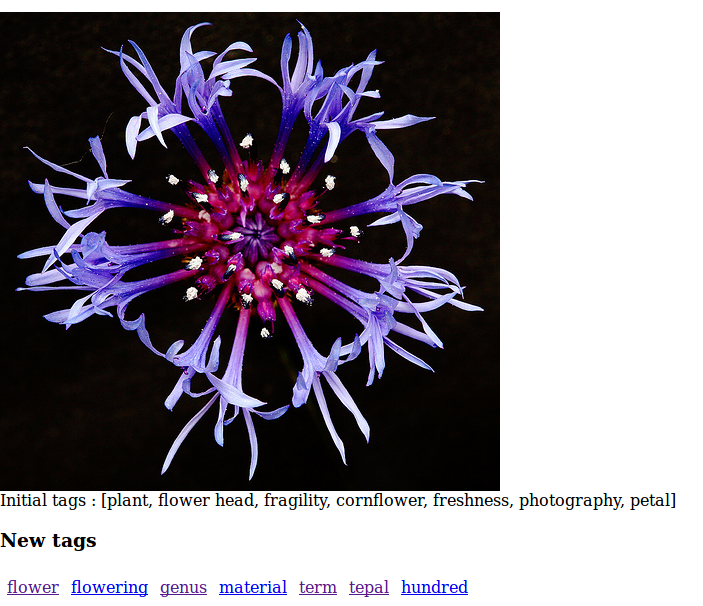
\includegraphics[scale=0.6]{./prim/exampleEval}
% section sample_image_to_evaluate (end)
\end{document}